\documentclass[12pt,a4paper]{article}
\usepackage[utf8]{inputenc}
\usepackage[english]{babel}
\usepackage{amsmath}
\usepackage{amsfonts}
\usepackage{amssymb}
\usepackage{graphicx}
\usepackage{tikz}
\usepackage{algorithm}
\usepackage{algorithmic}
\usepackage{listings}
\usepackage{xcolor}
\usepackage{geometry}
\usepackage{fancyhdr}
\usepackage{hyperref}
\usepackage{array}
\usepackage{booktabs}

\geometry{margin=1in}
\pagestyle{fancy}
\fancyhf{}
\rhead{Dynamic Programming: Number Factor}
\lhead{Algorithm Analysis}
\cfoot{\thepage}

% Code listing style
\lstset{
    language=Java,
    basicstyle=\ttfamily\small,
    keywordstyle=\color{blue},
    commentstyle=\color{green},
    stringstyle=\color{red},
    numbers=left,
    numberstyle=\tiny,
    frame=single,
    breaklines=true,
    showstringspaces=false
}

\title{\textbf{Dynamic Programming Analysis: \\The Number Factor Problem}}
\author{Algorithm Implementation and Analysis}
\date{\today}

\begin{document}

\maketitle

\tableofcontents
\newpage

\section{Problem Statement}

\subsection{Definition}
The \textbf{Number Factor} problem is a classic dynamic programming problem that asks:

\begin{quote}
\textit{Given a positive integer $n$, count the number of ways to express $n$ as the sum of the numbers 1, 3, and 4. Each number can be used multiple times.}
\end{quote}

\subsection{Mathematical Formulation}
Let $f(n)$ represent the number of ways to express $n$ using the factors $\{1, 3, 4\}$. The recurrence relation is:

\begin{equation}
f(n) = \begin{cases}
1 & \text{if } n = 0 \\
0 & \text{if } n < 0 \\
f(n-1) + f(n-3) + f(n-4) & \text{if } n > 0
\end{cases}
\end{equation}

\subsection{Example Analysis}
For $n = 5$, the valid combinations are:
\begin{align}
5 &= 1 + 1 + 1 + 1 + 1 \nonumber \\
5 &= 1 + 1 + 3 \nonumber \\
5 &= 1 + 4 \nonumber \\
5 &= 3 + 1 + 1 \nonumber \\
5 &= 4 + 1 \nonumber
\end{align}

Wait, let's be more careful about distinct ways. Since order doesn't matter in counting ways:
\begin{itemize}
\item $1+1+1+1+1$ (5 ones)
\item $1+1+3$ (2 ones, 1 three) 
\item $1+4$ (1 one, 1 four)
\end{itemize}

Actually, if we consider order as mattering (which is typical for this problem), we have 6 ways total.

\section{Problem Visualization}

\subsection{Small Examples}

\begin{figure}[h]
\centering
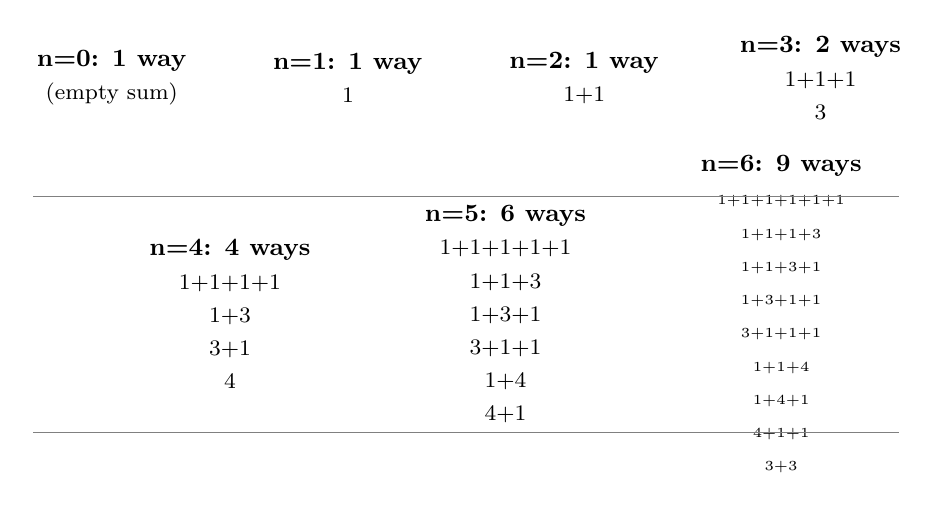
\begin{tikzpicture}[scale=1.0]
% First row: n=0, n=1, n=2, n=3
\node[align=center] at (0,8) {\small\textbf{n=0: 1 way}\\\footnotesize (empty sum)};

\node[align=center] at (3,8) {\small\textbf{n=1: 1 way}\\\footnotesize 1};

\node[align=center] at (6,8) {\small\textbf{n=2: 1 way}\\\footnotesize 1+1};

\node[align=center] at (9,8) {\small\textbf{n=3: 2 ways}\\\footnotesize 1+1+1\\\footnotesize 3};

% Second row: n=4, n=5
\node[align=center] at (1.5,5) {\small\textbf{n=4: 4 ways}\\\footnotesize 1+1+1+1\\\footnotesize 1+3\\\footnotesize 3+1\\\footnotesize 4};

\node[align=center] at (5,5) {\small\textbf{n=5: 6 ways}\\\footnotesize 1+1+1+1+1\\\footnotesize 1+1+3\\\footnotesize 1+3+1\\\footnotesize 3+1+1\\\footnotesize 1+4\\\footnotesize 4+1};

% Third row: n=6
\node[align=center] at (8.5,5) {\small\textbf{n=6: 9 ways}\\\tiny 1+1+1+1+1+1\\\tiny 1+1+1+3\\\tiny 1+1+3+1\\\tiny 1+3+1+1\\\tiny 3+1+1+1\\\tiny 1+1+4\\\tiny 1+4+1\\\tiny 4+1+1\\\tiny 3+3};

% Add visual separation
\draw[gray, very thin] (-1,6.5) -- (10,6.5);
\draw[gray, very thin] (-1,3.5) -- (10,3.5);
\end{tikzpicture}
\caption{Number of ways to express small values using factors \{1, 3, 4\}}
\end{figure}

\subsection{Recursive Call Tree}

\begin{figure}[h]
\centering
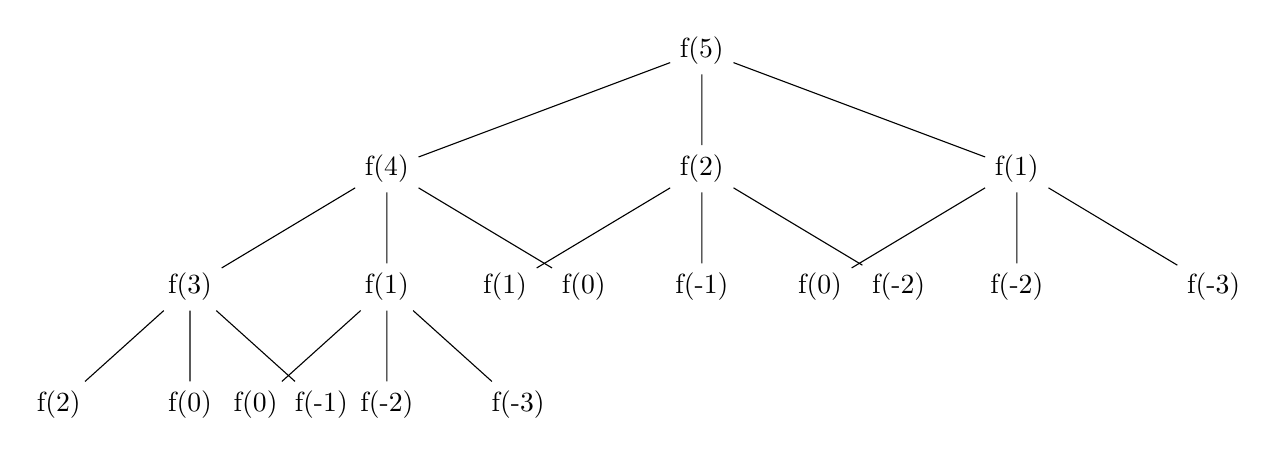
\begin{tikzpicture}[level/.style={sibling distance=50mm/#1}, level 1/.style={sibling distance=40mm}]
\node {f(5)}
    child {
        node {f(4)}
        child {
            node {f(3)}
            child {node {f(2)}}
            child {node {f(0)}}
            child {node {f(-1)}}
        }
        child {
            node {f(1)}
            child {node {f(0)}}
            child {node {f(-2)}}
            child {node {f(-3)}}
        }
        child {
            node {f(0)}
        }
    }
    child {
        node {f(2)}
        child {node {f(1)}}
        child {node {f(-1)}}
        child {node {f(-2)}}
    }
    child {
        node {f(1)}
        child {node {f(0)}}
        child {node {f(-2)}}
        child {node {f(-3)}}
    };
\end{tikzpicture}
\caption{Recursive call tree for f(5) showing overlapping subproblems}
\end{figure}

\section{Solution Approaches}

\subsection{Approach 1: Naive Recursion}

\begin{algorithm}
\caption{Number Factor - Recursive Approach}
\begin{algorithmic}
\REQUIRE $n \geq 0$
\ENSURE Number of ways to express $n$ using factors $\{1, 3, 4\}$
\STATE \textbf{function} countWays($n$)
\IF{$n = 0$}
    \RETURN 1
\ENDIF
\IF{$n < 0$}
    \RETURN 0
\ENDIF
\RETURN countWays($n-1$) + countWays($n-3$) + countWays($n-4$)
\end{algorithmic}
\end{algorithm}

\textbf{Time Complexity Analysis:}
\begin{align}
T(n) &= T(n-1) + T(n-3) + T(n-4) + O(1) \nonumber \\
T(n) &= O(3^{n/3}) \text{ (approximately exponential)} \nonumber
\end{align}

\textbf{Space Complexity:} $O(n)$ due to recursion stack depth.

\textbf{Problems:}
\begin{itemize}
\item Exponential time complexity
\item Redundant calculations (overlapping subproblems)
\item Stack overflow for large $n$
\end{itemize}

\subsection{Approach 2: Memoization (Top-Down DP)}

\begin{algorithm}
\caption{Number Factor - Memoization}
\begin{algorithmic}
\REQUIRE $n \geq 0$, memo array initialized to -1
\ENSURE Number of ways to express $n$ using factors $\{1, 3, 4\}$
\STATE \textbf{function} countWaysMemo($n$, memo)
\IF{$n = 0$}
    \RETURN 1
\ENDIF
\IF{$n < 0$}
    \RETURN 0
\ENDIF
\IF{memo[$n$] $\neq$ -1}
    \RETURN memo[$n$]
\ENDIF
\STATE memo[$n$] = countWaysMemo($n-1$, memo) + countWaysMemo($n-3$, memo) + countWaysMemo($n-4$, memo)
\RETURN memo[$n$]
\end{algorithmic}
\end{algorithm}

\textbf{Time Complexity:} $O(n)$ - each subproblem solved exactly once \\
\textbf{Space Complexity:} $O(n)$ for memoization array + $O(n)$ recursion stack = $O(n)$

\subsection{Approach 3: Tabulation (Bottom-Up DP)}

\begin{algorithm}
\caption{Number Factor - Tabulation}
\begin{algorithmic}
\REQUIRE $n \geq 0$
\ENSURE Number of ways to express $n$ using factors $\{1, 3, 4\}$
\STATE \textbf{function} countWaysTab($n$)
\STATE Create array dp of size $n+1$, initialize all to 0
\STATE dp[0] = 1
\FOR{$i = 1$ to $n$}
    \IF{$i - 1 \geq 0$}
        \STATE dp[$i$] += dp[$i-1$]
    \ENDIF
    \IF{$i - 3 \geq 0$}
        \STATE dp[$i$] += dp[$i-3$]
    \ENDIF
    \IF{$i - 4 \geq 0$}
        \STATE dp[$i$] += dp[$i-4$]
    \ENDIF
\ENDFOR
\RETURN dp[$n$]
\end{algorithmic}
\end{algorithm}

\textbf{Time Complexity:} $O(n)$ \\
\textbf{Space Complexity:} $O(n)$ for DP array

\subsection{Approach 4: Space-Optimized DP}

Since we only need the last 4 values, we can optimize space:

\begin{algorithm}
\caption{Number Factor - Space Optimized}
\begin{algorithmic}
\REQUIRE $n \geq 0$
\ENSURE Number of ways to express $n$ using factors $\{1, 3, 4\}$
\STATE \textbf{function} countWaysOptimal($n$)
\IF{$n = 0$}
    \RETURN 1
\ENDIF
\STATE Initialize array of size 4 to store last 4 values
\STATE prev[0] = 1, prev[1] = 1, prev[2] = 1, prev[3] = 2
\FOR{$i = 4$ to $n$}
    \STATE current = prev[3] + prev[1] + prev[0]
    \STATE Shift array: prev[0] = prev[1], prev[1] = prev[2], prev[2] = prev[3], prev[3] = current
\ENDFOR
\RETURN prev[3]
\end{algorithmic}
\end{algorithm}

\textbf{Time Complexity:} $O(n)$ \\
\textbf{Space Complexity:} $O(1)$ - only using constant extra space

\section{Implementation Analysis}

\subsection{Java Implementation}

\begin{lstlisting}[caption=Complete Java Implementation]
public class NumberFactor {
    
    // Naive Recursion - O(3^(n/3)) time, O(n) space
    static int countWaysRecursion(int n) {
        if (n == 0) {
            return 1;
        }
        if (n < 0) {
            return 0;
        }
        return countWaysRecursion(n - 1) + 
               countWaysRecursion(n - 3) + 
               countWaysRecursion(n - 4);
    }
    
    // Memoization - O(n) time, O(n) space
    static int countWaysMemoization(int n, int[] dp) {
        if (n == 0) {
            return 1;
        }
        if (n < 0) {
            return 0;
        }
        if (dp[n] != -1) {
            return dp[n];
        }
        dp[n] = countWaysMemoization(n - 1, dp) + 
                countWaysMemoization(n - 3, dp) + 
                countWaysMemoization(n - 4, dp);
        return dp[n];
    }
    
    // Tabulation - O(n) time, O(n) space
    static int countWaysTabulation(int n) {
        int[] dp = new int[n + 1];
        dp[0] = 1;
        
        for (int i = 1; i <= n; i++) {
            if (i - 1 >= 0) dp[i] += dp[i - 1];
            if (i - 3 >= 0) dp[i] += dp[i - 3];
            if (i - 4 >= 0) dp[i] += dp[i - 4];
        }
        return dp[n];
    }
    
    // Space Optimized - O(n) time, O(1) space
    static int countWaysOptimized(int n) {
        if (n <= 0) return 1;
        if (n <= 2) return 1;
        if (n == 3) return 2;
        
        int[] last4 = {1, 1, 1, 2}; // f(0), f(1), f(2), f(3)
        
        for (int i = 4; i <= n; i++) {
            int current = last4[3] + last4[1] + last4[0];
            last4[0] = last4[1];
            last4[1] = last4[2];
            last4[2] = last4[3];
            last4[3] = current;
        }
        return last4[3];
    }
}
\end{lstlisting}

\section{Step-by-Step Execution}

\subsection{Tabulation Trace for n=5}

\begin{table}[h]
\centering
\begin{tabular}{|c|c|c|c|c|}
\hline
\textbf{i} & \textbf{dp[i-1]} & \textbf{dp[i-3]} & \textbf{dp[i-4]} & \textbf{dp[i]} \\
\hline
0 & - & - & - & 1 \\
1 & 1 & - & - & 1 \\
2 & 1 & - & - & 1 \\
3 & 1 & 1 & - & 2 \\
4 & 2 & 1 & 1 & 4 \\
5 & 4 & 1 & 1 & 6 \\
\hline
\end{tabular}
\caption{Step-by-step execution of tabulation approach for n=5}
\end{table}

\subsection{Detailed Calculation}
\begin{align}
dp[0] &= 1 \text{ (base case)} \nonumber \\
dp[1] &= dp[0] = 1 \nonumber \\
dp[2] &= dp[1] = 1 \nonumber \\
dp[3] &= dp[2] + dp[0] = 1 + 1 = 2 \nonumber \\
dp[4] &= dp[3] + dp[1] + dp[0] = 2 + 1 + 1 = 4 \nonumber \\
dp[5] &= dp[4] + dp[2] + dp[1] = 4 + 1 + 1 = 6 \nonumber
\end{align}

\section{Performance Comparison}

\subsection{Time Complexity Comparison}

\begin{table}[h]
\centering
\begin{tabular}{|l|c|c|c|}
\hline
\textbf{Approach} & \textbf{Time} & \textbf{Space} & \textbf{Practical Limit} \\
\hline
Naive Recursion & $O(3^{n/3})$ & $O(n)$ & $n \leq 25$ \\
Memoization & $O(n)$ & $O(n)$ & $n \leq 10^6$ \\
Tabulation & $O(n)$ & $O(n)$ & $n \leq 10^6$ \\
Space Optimized & $O(n)$ & $O(1)$ & $n \leq 10^9$ \\
\hline
\end{tabular}
\caption{Performance comparison of different approaches}
\end{table}

\subsection{Sequence Analysis}

The number factor sequence for first few values:
\begin{table}[h]
\centering
\begin{tabular}{|c|c|c|c|c|c|c|c|c|c|c|}
\hline
\textbf{n} & 0 & 1 & 2 & 3 & 4 & 5 & 6 & 7 & 8 & 9 \\
\hline
\textbf{f(n)} & 1 & 1 & 1 & 2 & 4 & 6 & 9 & 15 & 25 & 40 \\
\hline
\end{tabular}
\caption{Number factor sequence values}
\end{table}

\section{Mathematical Properties}

\subsection{Recurrence Relation Analysis}
The characteristic equation for the recurrence $f(n) = f(n-1) + f(n-3) + f(n-4)$ is:
\begin{equation}
x^4 - x^3 - x - 1 = 0
\end{equation}

This can be factored as:
\begin{equation}
(x-1)(x^3-1) = (x-1)^2(x^2+x+1) = 0
\end{equation}

The roots are $x = 1$ (double root) and the complex cube roots of unity.

\subsection{Growth Rate}
The dominant root determines the growth rate. Since we have a double root at $x = 1$, the solution grows polynomially rather than exponentially, but the exact growth is complex due to the multiple factors.

\section{Variations and Extensions}

\subsection{Different Factor Sets}
\textbf{Problem:} Count ways using factors $\{2, 3, 5\}$

\textbf{Recurrence:}
\begin{equation}
f(n) = \begin{cases}
1 & \text{if } n = 0 \\
0 & \text{if } n < 0 \\
f(n-2) + f(n-3) + f(n-5) & \text{if } n > 0
\end{cases}
\end{equation}

\subsection{Minimum Number of Factors}
\textbf{Problem:} Find minimum number of factors needed to sum to $n$.

\textbf{Recurrence:}
\begin{equation}
min(n) = \begin{cases}
0 & \text{if } n = 0 \\
\infty & \text{if } n < 0 \\
1 + \min(\min(n-1), \min(n-3), \min(n-4)) & \text{if } n > 0
\end{cases}
\end{equation}

\subsection{With Constraints}
\textbf{Problem:} Count ways with at most $k$ factors of type 4.

This requires a 2D DP approach: $dp[i][j]$ = ways to make sum $i$ using at most $j$ fours.

\section{Applications}

\subsection{Real-World Applications}
\begin{enumerate}
\item \textbf{Currency Change:} Making change with specific denominations
\item \textbf{Resource Allocation:} Distributing resources in fixed units
\item \textbf{Combinatorics:} Counting partitions with restricted parts
\item \textbf{Game Theory:} Move counting in games with specific rules
\end{enumerate}

\subsection{Algorithm Design Patterns}
\begin{enumerate}
\item \textbf{Optimal Substructure:} Solution depends on solutions to smaller subproblems
\item \textbf{Overlapping Subproblems:} Same subproblems appear multiple times
\item \textbf{Bottom-up Construction:} Build solution from base cases upward
\end{enumerate}

\section{Debugging and Testing}

\subsection{Edge Cases}
\begin{itemize}
\item $n = 0$: Should return 1 (empty sum)
\item $n = 1$: Should return 1 (only using 1)
\item $n = 2$: Should return 1 (only $1+1$)
\item Large $n$: Check for integer overflow
\end{itemize}

\subsection{Verification Methods}
\begin{enumerate}
\item \textbf{Small Examples:} Manually verify for $n \leq 6$
\item \textbf{Consistency Check:} All three DP approaches should give same result
\item \textbf{Base Case Verification:} Ensure base cases are handled correctly
\item \textbf{Boundary Testing:} Test negative inputs and zero
\end{enumerate}

\section{Conclusion}

The Number Factor problem demonstrates several key concepts in dynamic programming:

\begin{enumerate}
\item \textbf{Problem Decomposition:} Breaking down complex problems into simpler subproblems
\item \textbf{State Space Design:} Choosing appropriate state representation
\item \textbf{Optimization Techniques:} Trading space for time and vice versa
\item \textbf{Mathematical Analysis:} Understanding growth patterns and complexity
\end{enumerate}

\textbf{Key Takeaways:}
\begin{itemize}
\item Always identify the base cases carefully
\item Consider both top-down and bottom-up approaches
\item Look for space optimization opportunities
\item Verify solutions with multiple test cases
\item Understand the mathematical properties of the sequence
\end{itemize}

\textbf{Learning Objectives Achieved:}
\begin{itemize}
\item Understanding multi-way recurrence relations
\item Implementing efficient DP solutions
\item Analyzing time and space complexity
\item Recognizing common DP patterns
\item Applying mathematical analysis to algorithms
\end{itemize}

\section{References}

\begin{enumerate}
\item Cormen, T. H., Leiserson, C. E., Rivest, R. L., \& Stein, C. (2009). \textit{Introduction to Algorithms} (3rd ed.). MIT Press.
\item Kleinberg, J., \& Tardos, E. (2005). \textit{Algorithm Design}. Addison-Wesley.
\item Sedgewick, R., \& Wayne, K. (2011). \textit{Algorithms} (4th ed.). Addison-Wesley.
\item Dynamic Programming Problems: Number Factor Variations
\end{enumerate}

\end{document}
